% Editable native annotations around unchanged verified IDE photographs.
\par
\begin{figure}[htbp]
  \centering
  \newsavebox{\MARScborheadregistersBox}
  \sbox{\MARScborheadregistersBox}{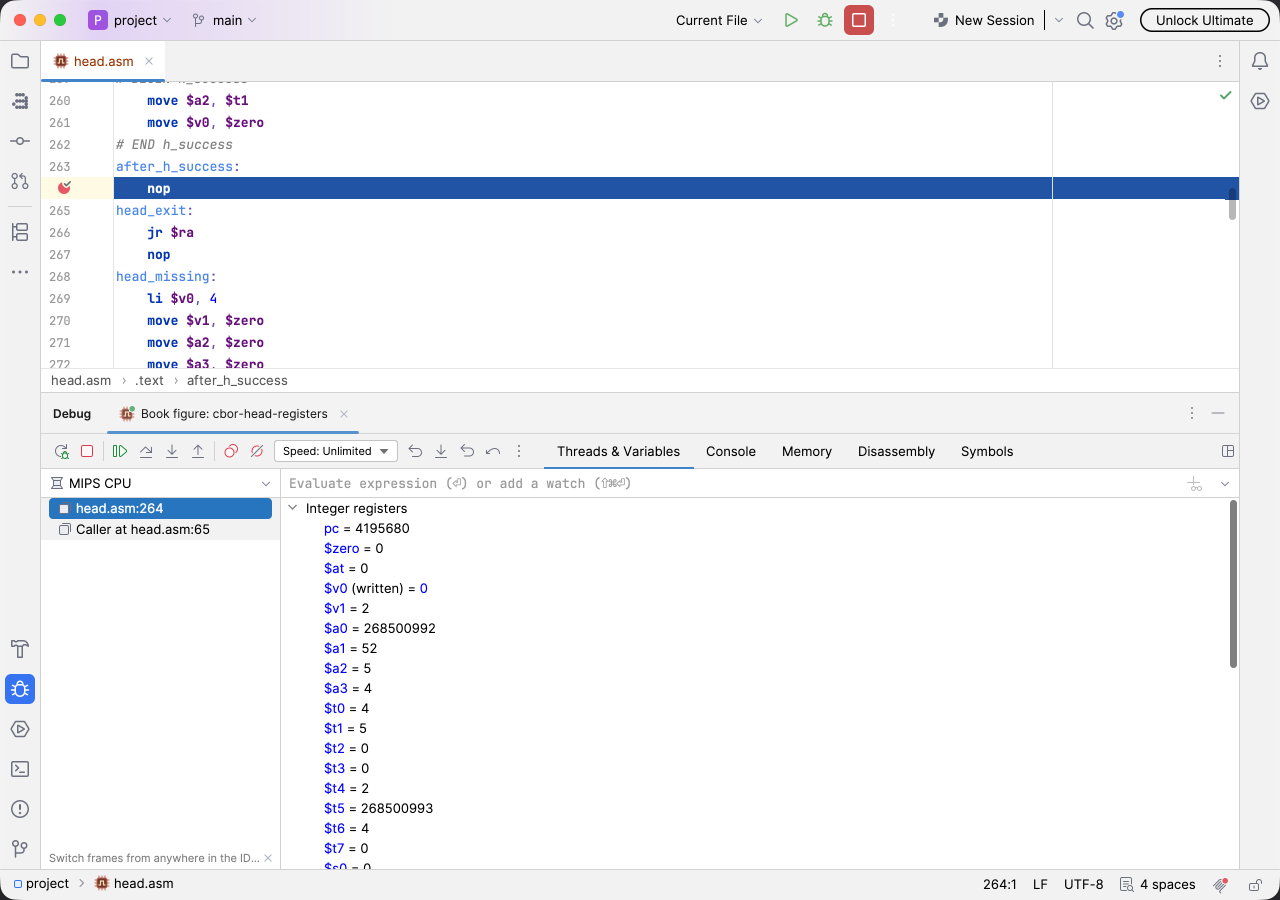
\includegraphics[artifact]{book/captures/032-cbor-telemetry/head-fields/registers.png}}
  \newsavebox{\MARScborheadsourceBox}
  \sbox{\MARScborheadsourceBox}{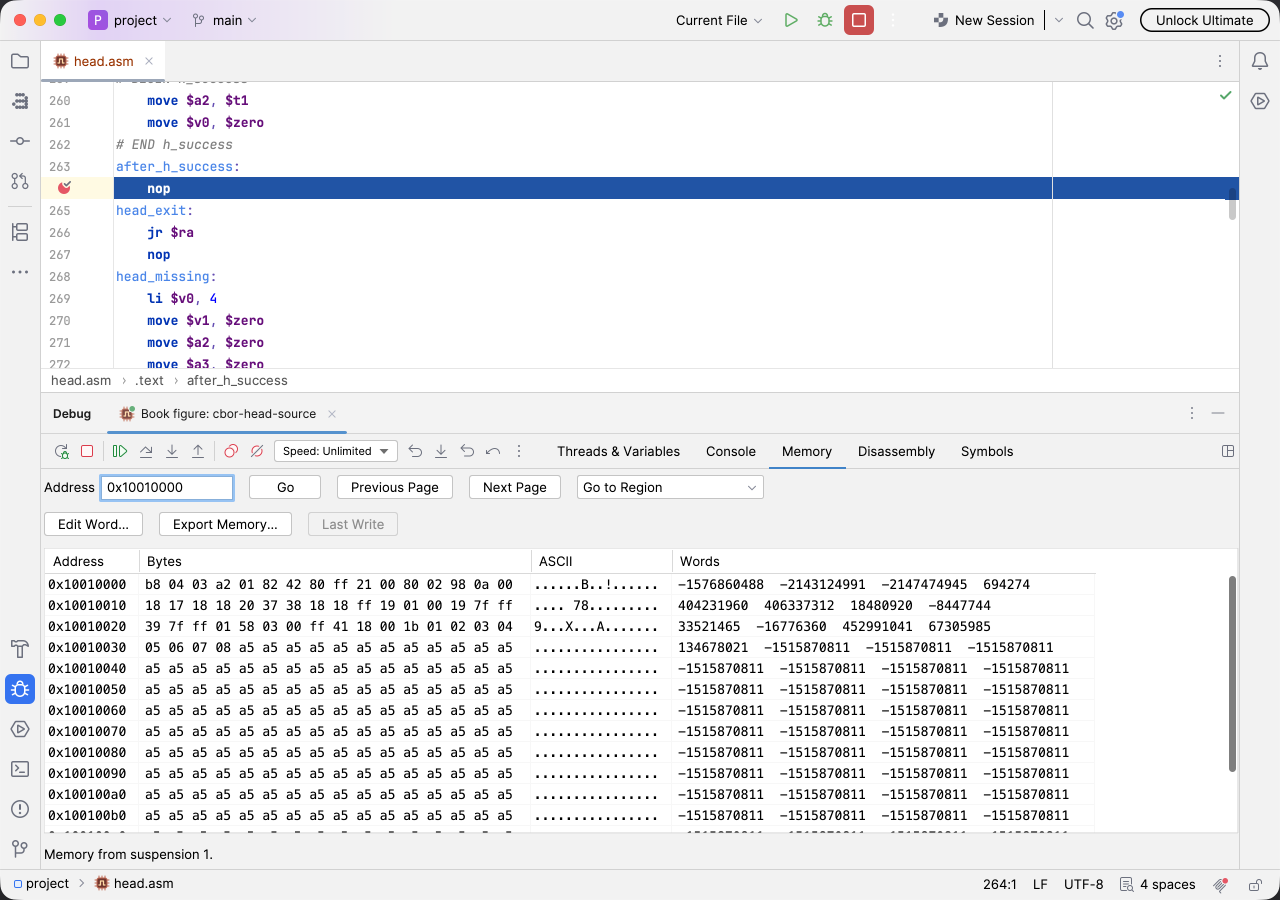
\includegraphics[artifact]{book/captures/032-cbor-telemetry/head-fields/source.png}}
  \edef\MARScborheadsourceLeft{\the\dimexpr0.036718750\wd\MARScborheadregistersBox\relax}
  \edef\MARScborheadsourceBottom{\the\dimexpr0.774444444\ht\MARScborheadregistersBox\relax}
  \edef\MARScborheadsourceRight{\the\dimexpr0.713281250\wd\MARScborheadregistersBox\relax}
  \edef\MARScborheadsourceTop{\the\dimexpr0.170000000\ht\MARScborheadregistersBox\relax}
  \edef\MARScborheadreturnsLeft{\the\dimexpr0.246093750\wd\MARScborheadregistersBox\relax}
  \edef\MARScborheadreturnsBottom{\the\dimexpr0.312222222\ht\MARScborheadregistersBox\relax}
  \edef\MARScborheadreturnsRight{\the\dimexpr0.553906250\wd\MARScborheadregistersBox\relax}
  \edef\MARScborheadreturnsTop{\the\dimexpr0.640000000\ht\MARScborheadregistersBox\relax}
  \edef\MARScborheadmeaningLeft{\the\dimexpr0.246093750\wd\MARScborheadregistersBox\relax}
  \edef\MARScborheadmeaningBottom{\the\dimexpr0.223333333\ht\MARScborheadregistersBox\relax}
  \edef\MARScborheadmeaningRight{\the\dimexpr0.553906250\wd\MARScborheadregistersBox\relax}
  \edef\MARScborheadmeaningTop{\the\dimexpr0.728888889\ht\MARScborheadregistersBox\relax}
  \edef\MARScborheadinputLeft{\the\dimexpr0.034375000\wd\MARScborheadsourceBox\relax}
  \edef\MARScborheadinputBottom{\the\dimexpr0.334444444\ht\MARScborheadsourceBox\relax}
  \edef\MARScborheadinputRight{\the\dimexpr0.584375000\wd\MARScborheadsourceBox\relax}
  \edef\MARScborheadinputTop{\the\dimexpr0.608888889\ht\MARScborheadsourceBox\relax}
  \begin{tikzpicture}[alt={Four details at after_h_success show the completed head instruction, success and width two, major type five and argument four, and input starting b8 04 before the map contents.}]
    \node[anchor=north west,inner sep=0,font=\small\bfseries] (source-title) at (6mm,0) {After completing the head result};
    \node[anchor=north west,inner sep=0] (source) at ([yshift=-1mm]source-title.south west) {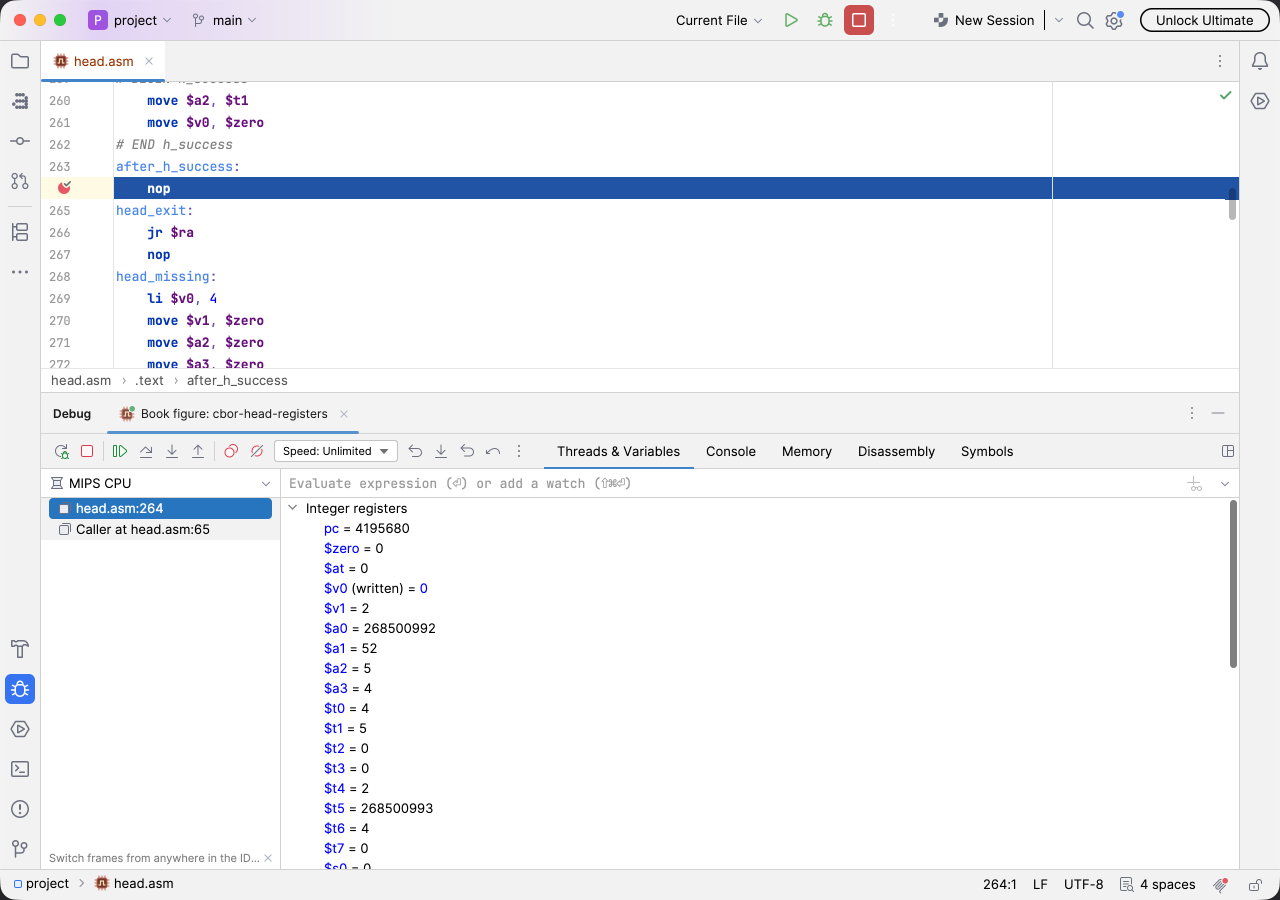
\includegraphics[width=0.54\linewidth,artifact,trim={\MARScborheadsourceLeft{} \MARScborheadsourceBottom{} \MARScborheadsourceRight{} \MARScborheadsourceTop{}},clip]{book/captures/032-cbor-telemetry/head-fields/registers.png}};
    \begin{scope}[shift={(source.south west)},x={($(source.south east)-(source.south west)$)},y={($(source.north west)-(source.south west)$)}]
      \draw[black,line width=0.7pt] (0.215625000,0.080000000) rectangle (0.384375000,0.520000000);
      \node[draw=black,fill=white,circle,inner sep=1.5pt,font=\footnotesize] at ($(0.215625000,0.520000000)+(-3mm,0)$) {1};
    \end{scope}
    \node[anchor=north west,inner sep=0,font=\small\bfseries] (returns-title) at ([yshift=-1mm]source.south west) {Success and consumed head width};
    \node[anchor=north west,inner sep=0] (returns) at ([yshift=-1mm]returns-title.south west) {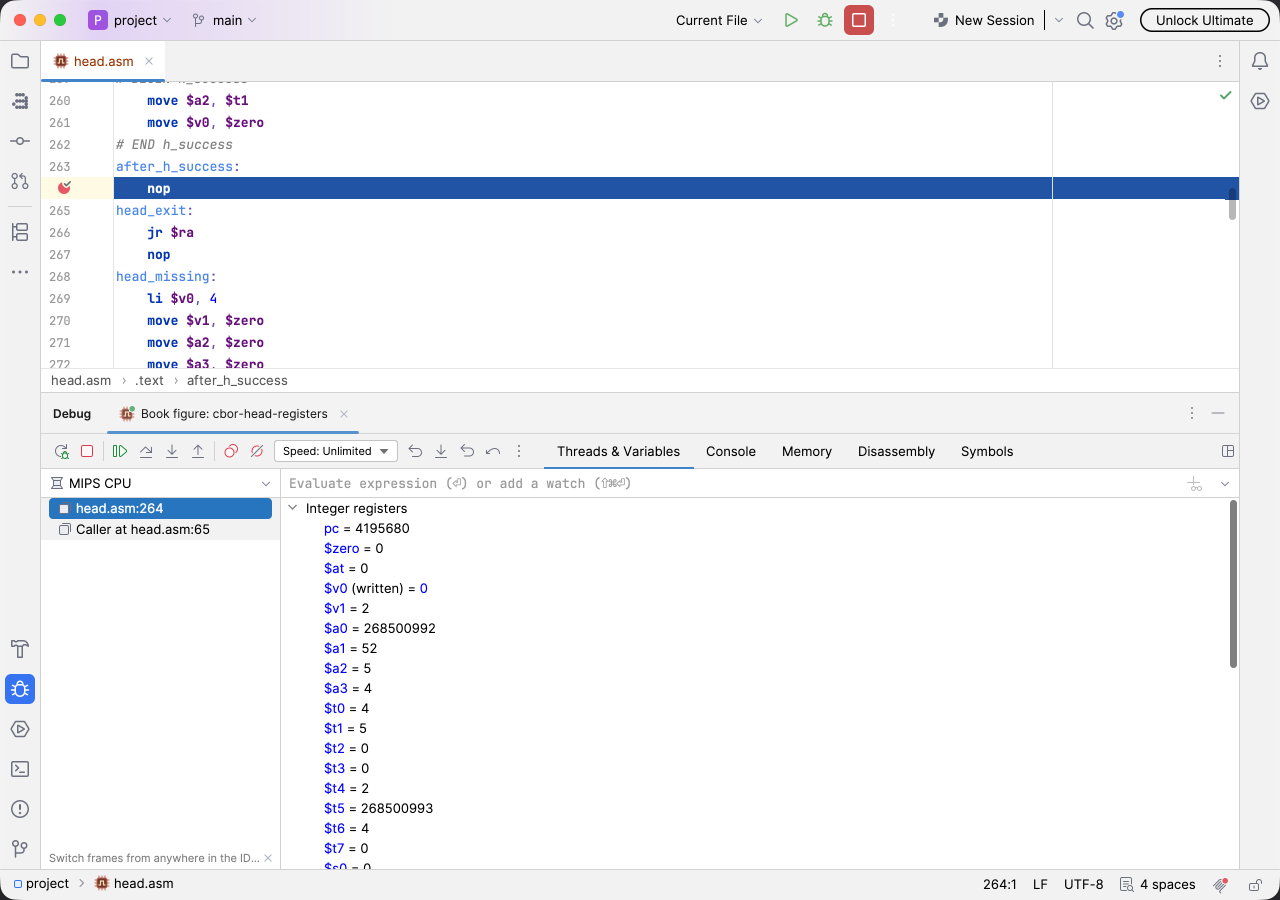
\includegraphics[width=0.48\linewidth,artifact,trim={\MARScborheadreturnsLeft{} \MARScborheadreturnsBottom{} \MARScborheadreturnsRight{} \MARScborheadreturnsTop{}},clip]{book/captures/032-cbor-telemetry/head-fields/registers.png}};
    \begin{scope}[shift={(returns.south west)},x={($(returns.south east)-(returns.south west)$)},y={($(returns.north west)-(returns.south west)$)}]
      \draw[black,line width=0.7pt] (0.023437500,0.023255814) rectangle (0.445312500,0.953488372);
      \node[draw=black,fill=white,circle,inner sep=1.5pt,font=\footnotesize] at ($(0.023437500,0.953488372)+(-3mm,0)$) {2};
    \end{scope}
    \node[anchor=north west,inner sep=0,font=\small\bfseries] (meaning-title) at ([yshift=-1mm]returns.south west) {Major type and its argument};
    \node[anchor=north west,inner sep=0] (meaning) at ([yshift=-1mm]meaning-title.south west) {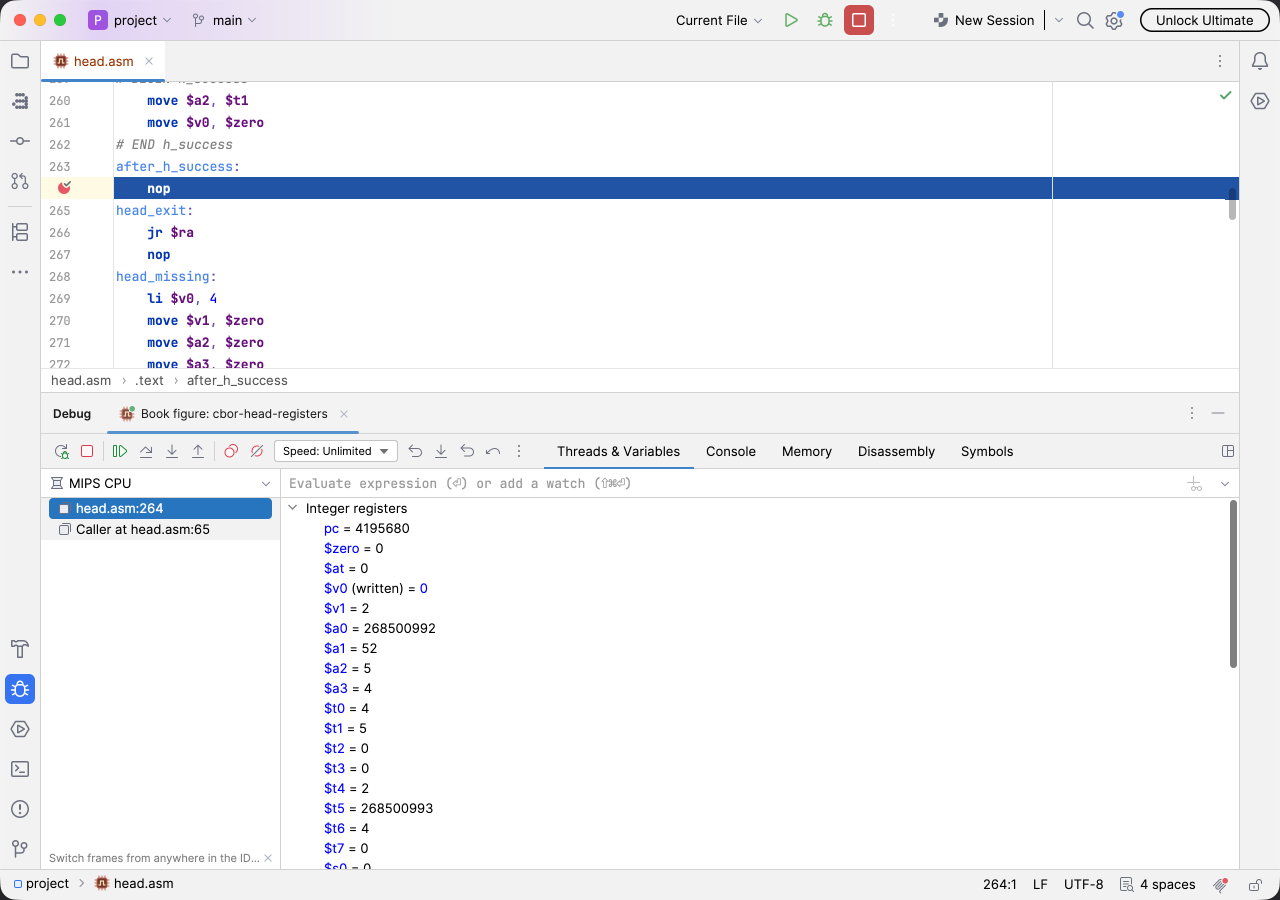
\includegraphics[width=0.48\linewidth,artifact,trim={\MARScborheadmeaningLeft{} \MARScborheadmeaningBottom{} \MARScborheadmeaningRight{} \MARScborheadmeaningTop{}},clip]{book/captures/032-cbor-telemetry/head-fields/registers.png}};
    \begin{scope}[shift={(meaning.south west)},x={($(meaning.south east)-(meaning.south west)$)},y={($(meaning.north west)-(meaning.south west)$)}]
      \draw[black,line width=0.7pt] (0.023437500,0.023255814) rectangle (0.230468750,0.953488372);
      \node[draw=black,fill=white,circle,inner sep=1.5pt,font=\footnotesize] at ($(0.023437500,0.953488372)+(-3mm,0)$) {3};
    \end{scope}
    \node[anchor=north west,inner sep=0,font=\small\bfseries] (input-title) at ([yshift=-1mm]meaning.south west) {Map head and the first following items};
    \node[anchor=north west,inner sep=0] (input) at ([yshift=-1mm]input-title.south west) {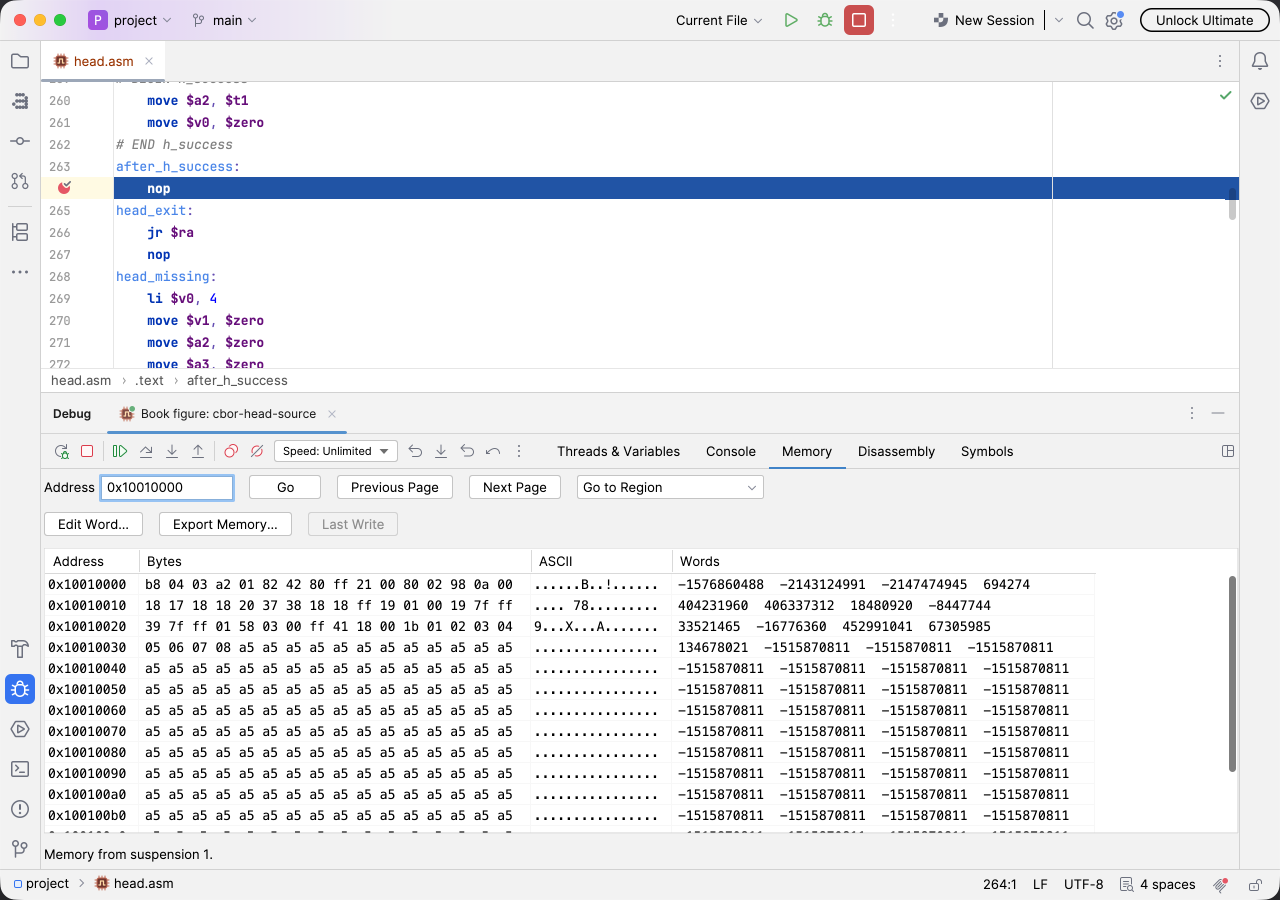
\includegraphics[width=0.84\linewidth,artifact,trim={\MARScborheadinputLeft{} \MARScborheadinputBottom{} \MARScborheadinputRight{} \MARScborheadinputTop{}},clip]{book/captures/032-cbor-telemetry/head-fields/source.png}};
    \begin{scope}[shift={(input.south west)},x={($(input.south east)-(input.south west)$)},y={($(input.north west)-(input.south west)$)}]
      \draw[black,line width=0.7pt] (0.194672131,0.078431373) rectangle (0.997950820,0.490196078);
      \node[draw=black,fill=white,circle,inner sep=1.5pt,font=\footnotesize] at ($(0,0.490196078)+(-3mm,0)$) {4};
    \end{scope}
  \end{tikzpicture}
  \par\smallskip
  \begin{minipage}{\linewidth}
    \small
    \begin{enumerate}
      \setlength{\itemsep}{0pt}
            \setlength{\parsep}{0pt}
      \item The stop at \texttt{after\_h\_success} precedes an observation \texttt{nop}. The head reader has completed its result assignments and will return through \texttt{head\_exit}.
      \item \texttt{v0 = 0} reports success. \texttt{v1 = 2} counts the initial byte and its one argument byte. It counts neither map pairs nor all bytes selected by the caller.
      \item \texttt{a2 = 5} identifies a map. \texttt{a3 = 4} is its pair count, so the map describes four keys and four corresponding values. The reader has decoded this head; it has not yet walked those items or accepted a telemetry record.
      \item The input begins \texttt{b8 04}. The upper three bits of \texttt{b8} give major type five; its lower five bits select a one-byte argument, whose value is four. This nonpreferred two-byte form is accepted on input by the local profile. The following \texttt{03 a2} begins a key and its value, not another byte of the root head.
    \end{enumerate}
  \end{minipage}
  \caption{A complete map head describes its children without validating them.}
  \label{capture:032-cbor-telemetry-head-fields}
  \label{cbor-head-fields}
\end{figure}
\par
